%%%%%%%%%%%%%%%%%%%%%%%%%%%%%%%%%%%%%%%%%%%%%%%%%%%%%%%%%%%%%%%%%%%%%%%%%%%%%%%%
%2345678901234567890123456789012345678901234567890123456789012345678901234567890
%        1         2         3         4         5         6         7         8

% \makeatletter
% \def\include@path{{./include/}}
% \makeatother

% \documentclass[A4, 10 pt, conference]{./include/ieeeconf/ieeeconf}  % Comment this line out if you need a4paper

\documentclass[a4paper, 10pt, conference]{IEEEtran}      % Use this line for a4 paper
% \documentclass[a4paper, 11pt]{report}      % Use this line for a4 paper


% \IEEEoverridecommandlockouts%                              % This command is only needed if
                                                           % you want to use the \thanks command

% \overrideIEEEmargins%                                      % Needed to meet printer requirements.

\makeatletter
\def\input@path{{./images/}{./include/}}
\makeatother
% \usepackage{adjustbox}
% \renewcommand{\IEEEtitletopspaceextra}{20pt}
% See the \addtolength command later in the file to balance the column lengths
% on the last page of the document

% The following packages can be found on http:\\www.ctan.org
\usepackage{graphicx} % for pdf, bitmapped graphics files
\usepackage{enumerate}
\usepackage{courier}
% \usepackage{enumitem} 
%\usepackage{epsfig} % for postscript graphics files
%\usepackage{mathptmx} % assumes new font selection scheme installed
%\usepackage{times} % assumes new font selection scheme installed
\usepackage{amsmath} % assumes amsmath package installed
\usepackage{amssymb}  % assumes amsmath package installed
\usepackage{bm}
\usepackage{listings}
% \usepackage{caption}
% \renewcommand{\lstlistingname}{Code}
\usepackage{tikz,ifthen,xstring,calc,pgfkeys,pgfopts}
% \usepackage{tikz-uml}
\usepackage{standalone}


\usepackage{wonhamautomata}
\usepackage{tikz}
\usetikzlibrary{positioning}
\usetikzlibrary{arrows}
\usetikzlibrary{fmbepics}
\usetikzlibrary{calc}
\usetikzlibrary{backgrounds}
\usetikzlibrary{fit}
\usetikzlibrary{shapes.symbols}
\usetikzlibrary{shapes.misc}
\usetikzlibrary{shapes.document}
\usetikzlibrary{shapes}

\tikzstyle{every picture}=[x=1em,y=1em,>=stealth,semithick]

\tikzstyle{document}=[shape=document % Warning shape and style overload
,minimum size=2em,draw,anchor=center,font=\smaller]
\tikzstyle{model}=[circle,minimum size=2em,draw,anchor=center]
\tikzstyle{realization}=[rectangle,minimum size=2em,draw,anchor=center]

\tikzstyle{actlb}=[above,inner sep=0pt,font=\relsize{-2}\strut]
\tikzstyle{actlb'}=[actlb,anchor=mid,fill=back]
\definecolor{tueblue}{rgb}{0.000,0.400,0.800}
\tikzstyle{act}=[->,shorten >=1pt,rounded corners]
\tikzstyle{iter}=[act,tueblue]
\tikzstyle{evalnode}=[draw,ellipse,tueblue,sloped,rotate=90]
\tikzstyle{evalconn}=[act,tueblue,below,font=\relsize{-1}]




\usetikzlibrary{positioning}
\usetikzlibrary{arrows}
\usetikzlibrary{shapes}
% \usetikzlibrary{fmbepics}
\usetikzlibrary{automata}

\tikzset{
    statesquaresup/.style={
           rectangle,
           rounded corners,
           draw=black, very thick,
           minimum height=2em,
           inner sep=2pt,
           text centered,
           fill=green!40
           },
}

\tikzset{
    statesquareimpl/.style={
           rectangle,
           rounded corners,
           draw=black, very thick,
           minimum height=2em,
           inner sep=2pt,
           text centered,
           fill=blue!20
           },
}

\tikzset{
    statesquarereq/.style={
           rectangle,
           rounded corners,
           draw=black, very thick,
           minimum height=2em,
           inner sep=2pt,
           text centered,
           fill=red!40
           },
}

% Define block styles
\tikzstyle{decision} = [diamond, draw, fill=orange!40, 
    text width=4.5em, text badly centered, inner sep=0pt, aspect=1.5, yshift=1cm]
\tikzstyle{block} = [rectangle, draw, fill=blue!20, 
    text width=5em, text centered, rounded corners, minimum height=4em]
\tikzstyle{line} = [draw, -latex']
\tikzstyle{cloud} = [draw, ellipse,fill=red!20, node distance=3cm,
    minimum height=2em]
\tikzstyle{decision answer}=[midway,left,color=black]
    
% \usepackage{wonhamautomata}
\usepackage{color}
\definecolor{tueblue}{rgb}{0.000,0.400,0.800}

\usepackage{todonotes}
\presetkeys{todonotes}{inline,fancyline}{}

\usepackage{url}
\usepackage[backend=biber, style=ieee,  sorting=none]{biblatex}
\addbibresource{ref.bib}
\usepackage[capitalise]{cleveref}

%\newcommand{\todo}[1]{{\textcolor{blue}{#1}}}
\newcommand{\spred}[1]{\textbf{#1}~$\downarrow$}
\newcommand{\epred}[1]{$\rightarrow$ \{ \textit{#1} \}}
\newcommand{\nepred}[1]{$\nrightarrow$~\{~\textit{#1}~\}}

\newcommand{\logand}{$\wedge$}
\newcommand{\logor}{$\vee$}
\newcommand{\logimplies}{$\Rightarrow$}
\newcommand{\lognot}{$\neg$}

\lstdefinelanguage{CIF}
{morekeywords={*,plant, def, location, marked, initial, edge, controllable, disc, bool, end, :},
sensitive=false,
morecomment=[l]{//},
morecomment=[s]{/*}{*/},
morestring=[b]",
}

\lstset{ 
  backgroundcolor=\color{white},   % choose the background color; you must add \usepackage{color} or \usepackage{xcolor}; should come as last argument
  basicstyle=\footnotesize,        % the size of the fonts that are used for the code
  breakatwhitespace=false,         % sets if automatic breaks should only happen at whitespace
  breaklines=true,                 % sets automatic line breaking
  captionpos=b,                    % sets the caption-position to bottom
  commentstyle=\color{green},    % comment style
  deletekeywords={...},            % if you want to delete keywords from the given language
  escapeinside={\%*}{*)},          % if you want to add LaTeX within your code
  extendedchars=true,              % lets you use non-ASCII characters; for 8-bits encodings only, does not work with UTF-8
  frame=single,                    % adds a frame around the code
  keepspaces=true,                 % keeps spaces in text, useful for keeping indentation of code (possibly needs columns=flexible)
  keywordstyle=\color{blue},       % keyword style
  % morekeywords={*,plant, def, location, marked, initial, edge, controllable, disc, bool},            % if you want to add more keywords to the set
  numbers=left,                    % where to put the line-numbers; possible values are (none, left, right)
  numbersep=5pt,                   % how far the line-numbers are from the code
  numberstyle=\tiny\color{black}, % the style that is used for the line-numbers
  rulecolor=\color{black},         % if not set, the frame-color may be changed on line-breaks within not-black text (e.g. comments (green here)) 
  showspaces=false,                % show spaces everywhere adding particular underscores; it overrides 'showstringspaces'
  showstringspaces=false,          % underline spaces within strings only
  showtabs=false,                  % show tabs within strings adding particular underscores
  stepnumber=2,                    % the step between two line-numbers. If it's 1, each line will be numbered
  stringstyle=\color{muave},     % string literal style
  tabsize=2,                     % sets default tabsize to 2 spaces
  title=\lstname                   % show the filename of files included with \lstinputlisting; also try caption instead of title
  % linewidth=0.6\columnwidth
}


\title{\LARGE \bf 
Supervisory Control Synthesis for Autonomous Robots\\
\large A Study Using an Autonomous Service Robot}

\author{J. Smit, Prof. dr. ir. H.P.J. Bruyninckx,\\dr.ir. M.J.G. van de Molengraft,  
dr.ir. J.M. van de Mortel - Fronczak}% <-this % stops a space
%\thanks{*This work was not supported by any organization}% <-this % stops a space
\thanks{$^{1}$A.A. Author and B.B. Author are with the Department of Mechanical Engineering, Eindhoven University of Technology, 5612 AZ Eindhoven, The Netherlands
        {\tt\small jorritsmit@gmail.com}}%
%\thanks{$^{2}$Bernard D. Researcheris with the Department of Electrical Engineering, Wright State University,
%        Dayton, OH 45435, USA
%        {\tt\small b.d.researcher@ieee.org}}%



\begin{document}

\graphicspath{{./images/}}

\maketitle
%\thispagestyle{empty}
%\pagestyle{empty}
\thispagestyle{plain}
\pagestyle{plain}

%%%%%%%%%%%%%%%%%%%%%%%%%%%%%%%%%%%%%%%%%%%%%%%%%%%%%%%%%%%%%%%%%%%%%%%%%%%%%%%%
\begin{abstract}

As shown in literature, supervisory control synthesis could provide numerous benefits in system design, e.g.\@ reducing time-to-market, and task execution, e.g.\@ ensuring safety requirements are met. 
However, supervisory control synthesis is usually not used in a dynamic environment such as autonomous robotics. 
The purpose of this paper, therefore, is to explore the limitations, benefits and application scope of supervisory control synthesis in autonomous robotics.
Using two case studies presented in this paper, we show that supervisory control synthesis and model based engineering provides us with a new methodology for designing and programming autonomous robots. 
This methodology reduces development time and manually made coding errors, through the use of modular en re-usable models of the robot and requirements, specifying its required behaviour.
Supervisory control synthesis is suited for high-level decision making and task- and safety requirements specification, but less suited for low level control of the robot.
Therefore, the case studies also explore the application scope of supervisory control synthesis for autonomous robots.
The application scope is defined as the range of abstraction levels supervisory control synthesis can be applied to in autonomous robots.\\
% Possible research and methods that can eliminate limitations to the application of supervisory control synthesis for autonomous robots are also presented.

\end{abstract}


%%%%%%%%%%%%%%%%%%%%%%%%%%%%%%%%%%%%%%%%%%%%%%%%%%%%%%%%%%%%%%%%%%%%%%%%%%%%%%%%

\section{INTRODUCTION}\label{sec:introduction}

Autonomous robots are a promising next step in robotics. They could help solve many of current major societal challenges. Examples include assistance at home\todo[disable]{ref}, in care centres\todo[disable]{ref}, but also in industrial environments~\cite{sup_navigation}.
However, the complicated dynamic environment these robots operate in and the complex actions they have to perform, make this a challenging field. 
Advancements in computing power and hardware have made autonomous robots increasingly capable of providing the complex tasks required to operate in these environments, but at the same time increasingly complex systems.\\ 
Since the introduction of the supervisory control theory of Ramadge and Wonham~\cite{original}, the benefits of supervisory control synthesis have been discussed and proven in numerous papers. Benefits relating to system design, as shown e.g.\@ in~\cite{themepark}, and benefits relating to task execution.
\todo[disable]{ref}

These benefits could help manage the aforementioned increase in complexity in autonomous robotics.\\

Improvements in system design that supervisory control synthesis can offer are illustrated in \cref{fig:TR_and_MB_SE_processes,fig:sup_se} from~\cite{Baeten2016}. 
The figures show the systems engineering design process from traditional to model-based with supervisory control theory included. 
The traditional SE design process and MBSE design process are represented in \cref{fig:TR_and_MB_SE_processes} for a system with a controller \(S\) and plant \(P\).
In traditional SE the requirements are tested on the realization of the design, without using models of the designs.
This is represented in \cref{fig:TR_and_MB_SE_processes} with the \textit{realize} arrow from design to realization.
For complex systems, time-to-market and errors can be reduced by testing the design before realizing it. 
The process of Model Based Systems Engineering (MBSE)~\cite{mbse}, also shown in \cref{fig:TR_and_MB_SE_processes}, uses models of \(S\) and \(P\) for that reason, and, among others,~\cite{themepark} demonstrates that it indeed improves time-to-market and reduces errors.
The next evolution of integrating models in the design process is using supervisory control synthesis of \(S\) from \(P\) and the models of the system requirements (\cref{fig:sup_se}).
Where the traditional SE process relies heavily on documentation, from defining the requirements to realizing a design, the models used in MBSE provide a more systematic and unambiguous specification of \(S\) and \(P\).
This makes working on large multi-disciplinary projects faster and easier.
Finally, using supervisory control synthesis on models of requirements guarantees that requirements are met, even in complex systems.
This reduces the reliance on documentation and testing even more and prevents errors created by the implementation phase of the requirements.\\

\begin{figure}
\begin{center}
\includestandalone[width=0.9\columnwidth]{./images/tikz/Traditional_and_MB_SE}

\scriptsize{
  \tikz[fmbe,baseline=(x.base)]{\node[document] (x) {$\phantom{X}$};} = documents
  \tikz[fmbe,baseline=(x.base)]{\node[model](x){$\phantom{Y}$};} = models
  \tikz[fmbe,baseline=(x.base)]{\node[realization](x){$\phantom{Z}$};} = realizations}
\end{center}
\caption{Traditional and model-based systems engineering processes}
  \label{fig:TR_and_MB_SE_processes}
\end{figure}


\begin{figure}[!h]
  \centering
  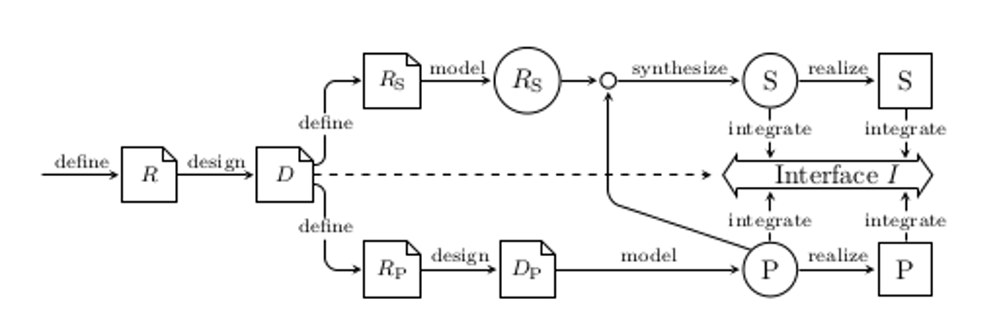
\includegraphics[width=\columnwidth]{sup_se.png}
  \caption{Supervisory control synthesis-based systems engineering process}\label{fig:sup_se}
\end{figure}
\newpage
Besides the above mentioned benefits relating to system design, supervisory control synthesis offers benefits in task execution as well.
Task execution benefits, in this paper, are a group of benefits relating to reductions in man-made errors when programming the robot.
The following guarantees supervisory synthesis offers, would have to be ensured by proper implementation of logic throughout the code, when not using supervisory control synthesis.
This approach, without using supervisory control synthesis, is sensitive to mistakes; incorrectly implementing the logic in just one place can cause unwanted behaviour.
Also, when the system changes, the logic has to be changed everywhere.
Supervisory control theory guarantees synthesis of a non-blocking, maximally permissive and controllable supervisor, as explained in \cref{sec:supervisory_control}.
These are useful when executing tasks, because it removes the ownership of these problems from the software developer to the supervisor.
Another benefit provided by supervisory control synthesis, somewhat specific to this paper, is the more straightforward implementation of concurrent task execution.
Traditionally, the software developer has to implement all the conditions regarding when a task can be executed, has to be interrupted or stopped, himself.
With supervisory control synthesis, however, the supervisor will block all tasks (or events) that violate the requirements.
Therefore, ensuring a task will never be executed untimely, as long as the requirements are specified correctly.\\

Despite the advantages of applying supervisory control theory to autonomous robots, there has been little research in the field. 
The research that has been done usually focusses on using supervisory control to govern the way robots interact with each other~\cite{sup_swarm}, using a human as supervisor~\cite{sup_human} or an autonomous robot operating in a relatively static environment~\cite{sup_navigation}.
This is understandable, because supervisory control has three limitations that seem to make it unsuitable for autonomous robots:

\begin{itemize}
  \item Supervisory control can only be applied to discrete-event systems.
  \item The synthesis of the supervisor is done off-line, so it cannot deal with the robot entering an unknown environment.
  \item Supervisory control theory assumes asynchronous and instantaneous task execution.
\end{itemize}

The purpose of this paper is to investigate these limitations, defining on what abstraction levels supervisory control synthesis can be applied, defined as the application scope, in autonomous robots and to explore the impact and benefits it can have.
Using the Amigo robot at the Eindhoven University of Technology, two case studies are presented. 
These case studies showcase the benefits of using supervisory control synthesis and the application scope of the theory to autonomous robotics. 
A method is proposed that not only presents a new beneficial way to control autonomous robots, but also show what is and what is not (yet) possible.\\

The paper is structured as follows. \Cref{sec:supervisory_control} provides some necessary background on supervisory control theory and discrete-event systems. It is followed by an explanation of the case studies in \cref{sec:case_studies}. The methodology and design choices are explained in \cref{sec:method}.
The results of applying the described method to these case studies are presented in \cref{sec:results}.
Finally, \cref{sec:conclusions} discusses the limitations of using supervisory control synthesis for autonomous robots and possible research that can eliminate them.\\
\section{SUPERVISORY CONTROL THEORY}\label{sec:supervisory_control}
Without going into too much detail, this section explains the topics of supervisory control synthesis and discrete-event systems.
It contains the necessary background information to understand the research described in this paper.\\
Supervisory control theory applies to a subset of systems called Discrete Event Systems (DES).
These systems are represented by discrete locations (states) and event-labelled transitions and can be modelled by automata.
Additionally, in extended automata, also (discrete) variables can be used.
An extended automaton allows to additionally augment the transitions with guards and updates.\\

An automaton \(G\) is formally described as follows:
\begin{equation}
  G = (L,V, E, \rightarrow, L_m , l_0 , \nu_0)
\end{equation}
with:
\begin{description}
  \item[\(L\)] a finite set of locations
  \item[\(V\)] a finite set of discrete variables
  \item[\(E\)] a finite set of events
  \item[\( \rightarrow\)] \(\subseteq L \times G(V) \times E \times U(V ) \times L\) the transition relation
  \item[\( L_m\)] the set of marked locations, \(L_m \subseteq L\)
  \item[\( l_0\)] the initial location, \(l_0 \in L\)
  \item[\( \nu_0\)] the initial valuation of the variables, \(\nu_0:V \rightarrow \lambda\) and \(\lambda\) is the set of all values\\
\end{description}

An example automaton is graphically depicted in \cref{fig:automaton}.\\[2ex]

\begin{figure}[!ht]
  \centering
  \begin{tikzpicture}[->,>=stealth',shorten >=1pt,auto,node distance=4cm,
                      semithick, every node/.style={scale=1.2}]
    % \tikzstyle{every state}=[fill=red,draw=none,text=white]

    \node[initial,state]      (1)                     {$l_1$};
    \node[state]              (2) [below right of=1]  {$l_2$};
    \node[state, accepting]   (3) [right of=1]  {$l_3$};

    \path (1) edge [bend left]          node [align=center] {$v_1 < 5$ \\ $e_1$} (3)
              edge [bend right]          node [align=center, left] {$e_3$ \\ $v_1 := v_1 +1$} (2)
          (2) edge [bend right]          node                {$e_4$} (3)
          (3) edge [bend left]         node                {$e_2$} (1);
  \end{tikzpicture}
  \caption{Graphic depiction of an automaton}\label{fig:automaton}
\end{figure}

with:
\begin{description}[\IEEEsetlabelwidth{\(e_1, e_2, e_3, e_4\)}]
  \item[\(l_1, l_2,l_3\)] the locations
  \item[\(v_1\)] the discrete variable
  \item[\(e_1, e_2, e_3, e_4\)] the events
  \item[\(l_3\)] the marked location
  \item[\(l_1\)] the initial location
  \item[\(v_1=0\)] the initial values of the variables
  \item[\(v_1 := v_1+1\)] the update of \(v_1\) done by event \(e_3\)
  \item[\(v_1 < 5\)] the guard for event \(e_1\)\\
\end{description}

A model of a DES usually consists of multiple automata, sharing variables and events, called a network of automata.\\

In supervisory control theory, an uncontrolled system that is modelled by these automata is called a plant. 
A distinction is made between controllable events, which can be controlled by the supervisor, and uncontrollable events, which cannot be controlled.
A button that needs to be pressed by a user, for example, is an uncontrollable event.
When combined with a set of requirements, supervisory control theory provides a way to automatically synthesize a supervisor.
These requirements can, for example, be a set of safety requirements or process requirements.
Safety requirements prevent dangerous situations from occurring, e.g.\@ the robot colliding with its environment or itself.
Process requirements ensure a certain order of events, e.g.\@ not releasing an object before reaching the table on which the object is supposed to be placed.
The requirements can be modelled in the same way as the plant, with an automaton, and can refer to the plant variables and locations.
It can also be modelled as a state-based expression, a requirement specified in terms of conditions of a state.
Where a guard in an automaton based requirement would block an event from happening based on a condition of a variable, a state based expression prescribes in what state the system cannot be in, or what value a variable cannot have.
While the same result can be obtained with an automaton based requirement, a state-based expression can offer a more intuitive way to describe requirements.  
The synthesized supervisor then disables events that would lead to a violation of these requirements.\\

There are a few important benefits, applicable to this research, that follow from the following.\\

\begin{LaTeXdescription}
\item[Separation] The requirements and plant can be described separately. This separation means adjustments to requirements or plant only have to be applied locally. Synthesis will take care of the knock-on effects of these changes. In conventional programming changing a simple requirement would not only involve tedious work in many different places in the code, the software developer also has to think of all the implications of the change himself and apply them correctly. This separation will make developing easier and faster.\\
\item[Modular design] The method proposed in \cref{sec:method} uses separate modules for groups of requirements, e.g.\@ skill requirements and task requirements. An example of a skill requirement used in this paper, is the grab skill, described in \cref{sec:method}. Only when needed in a certain task this skill can be included, thus creating a modular system.\\
\item[Re-usability] The models of the requirements and the robot can be applied to new tasks, or even new robots, without many adjustments. Because the robot model contains general components used in robots, e.g.\@ arms, the robot model can mostly stay the same when using a different robot. Only the intermittent communication layer between the supervisor and the robot, is robot specific.\\

\end{LaTeXdescription}

As mentioned before, supervisory control theory does not only provide benefits related to system design (\cref{sec:introduction}), but also related to task execution.
The synthesized supervisor has two useful properties related to task execution: non-blockingness and the guarantee that all events that would lead to a violation of the requirements are blocked.
A non-blocking supervisor blocks the execution of every event that would lead to a system state from which no marked state \(L_m\) can be reached.

These properties are useful, because without the use of supervisory control synthesis, the software developer would have to create these properties with logic in the code.
Removing the ownership of this issue to the supervisor can prevent unwanted behaviour when changes have to be made to related parts of the system.
The developer could forget to change the logic in all the related parts and the system can reach a blocking state or violate the requirements.\\

Supervisory control synthesis also guarantees a maximally permissive and controllable supervisor.
Maximal permissiveness assures that only those events that could lead to a violation of the requirements or the non-blockingness principle, are blocked by the supervisor.
Controllability refers to the fact that the supervisor only blocks controllable events.\\ 


When synthesizing one supervisor for large systems with many components, an effect occurs called state-space explosion. 
This kind of supervisor is called a monolithic supervisor and since it has to account for all possible state combinations of the components and block according to all the requirements, it becomes very large and takes a long time to synthesize.
There are different synthesis techniques that can circumvent this problem, i.e.\@ modular~\cite{modular} or hierarchical~\cite{hierachical} synthesis and although they were not necessary for the case studies in this research, they could prove useful when increasing the scope and complexity of the supervisor.\\

\todo[disable]{talk about no existence of non-blockingness in dynamic environment}


\section{CASE STUDIES}\label{sec:case_studies}
\Cref{sec:introduction} states the main contribution and purpose of this paper:
to investigate the limitations, benefits and application scope of supervisory control synthesis for autonomous robots.
To this end, two case studies were designed to showcase what supervisory control can contribute in the field of autonomous robotics.\\

As discussed in \cref{sec:introduction}, the benefits of supervisory control synthesis can be classified into two main categories: system design and task execution. 
Further on in \cref{sec:supervisory_control}, these categories were expanded on.
For systems design, aspects related to separation, modularity and re-usability were discussed.
The properties of the synthesized supervisor, non-blockingness and no violation of the requirements, are benefits in the task execution category.
The case studies presented here show the extent to which these benefits and principles can be applied to autonomous robots, using the method described in \cref{sec:method}.\\

The robot used for the case studies, is the Amigo robot, see~\cite{amigo_rop,amigo_ros,amigo_paper}. 
This is an autonomous service robot developed and maintained at the Eindhoven University of Technology in the Control Systems Technology Group. It competes in the RoboCup@Home league and has a functional system architecture and code, which can be found in the \texttt{tue\_robotics} repository~\cite{amigo_github}. 
This robot was chosen for the case studies, because the low-level control design was already in place and from there, it was possible to use supervisory control synthesis to control the robot with high-level commands. 
Also, the robot is controlled at task and skill level by a finite-state machine implementation in ROS using the SMACH library~\cite{smach}, which was thought to make interaction with the synthesized supervisor more straightforward.
The robot model, its requirements and the synthesized supervisor are created with the CIF 3 tool set~\cite{cif3}. CIF 3 is also developed and maintained at the Control Systems Technology Group.
CIF 3 can generate a C library~\cite{cif3_manual} implementation of the supervisor and this is leveraged to fuse the existing SMACH finite-state machines with the supervisor.
When the robot is being used without supervisor, a task is described by a SMACH finite state-machine.
In the case studies presented here, this task finite state-machine is replaced by a communication layer between the supervisor and the robot system architecture, called a wrapper. 
\Cref{fig:system_architecture} depicts the system architecture used for the case studies. \Cref{sec:method} provides a more detailed description of this architecture.\\

\begin{figure}[!ht]
\centering
% ->,>=stealth',
	\begin{tikzpicture}[node distance=2cm, auto,
                      semithick, text width=1.7cm, font=\footnotesize]
    % \node [circle, fill=black] (1){};
    % \node (2)[above of=1]{};
    % \node (3)[below of=1]{};

    \node[statesquaresup, align=left] (supervisor) {\textbf{Supervisor} \\
                                CIF 3};
    \node[statesquareimpl,left=0.4cm of supervisor, align=left] (smach) {\textbf{Wrapper} \\
                                              Communcation layer between the supervisor and existing system architecture};
    \node[statesquareimpl,above left=0.3cm and 0.3cm of smach, align=left] (skills) {\textbf{Robot skills} \\
                                               Robot abstraction layer of Amigo};
    \node[statesquareimpl,below left =0.3cm and 0.3cm of smach, align=left] (states) {\textbf{Robot states} \\
                                               SMACH skill specification of Amigo};
    \node[statesquarereq, align=left, above right=0.75cm and 0.5cm of supervisor] (req-safe) {\textbf{Requirements} \\
                                A CIF model of the safety requirements for Amigo};
    \node[statesquarereq, align=left, right=0.5cm of supervisor] (req-skill) {\textbf{Requirements} \\
                                A CIF model of the skill-specific requirements for Amigo};
    \node[statesquarereq, align=left, below right=0.75cm and 0.5cm of supervisor] (req-task) {\textbf{Requirements} \\
                                A CIF model of the task-specific requirements for Amigo};

    \draw [dashed] (-3.2,-9) -- (-3.2,9);

    % \draw [line, dashed] (2) -- (3);
    % \draw [line, ->] (1)  -- (smach);
    % \draw [line, ->] (1)  -- (supervisor);
    \draw [line, <->] (smach)  -- (supervisor);

    \draw [line] (skills)  -| (smach);
    \draw [line] (skills)  -- (states);
    \draw [line] (states)  -| (smach);
    \draw [line] (req-safe)  -| (supervisor);
    \draw [line] (req-skill)  -- (supervisor);
    \draw [line] (req-task)  -| (supervisor);

	\end{tikzpicture}
  \caption{System architecture}\label{fig:system_architecture}
\end{figure}

\subsection{CASE STUDY I:\@ PICK AND PLACE}\label{sec:cs1}
In this case study, Amigo navigates to a table with an object on it. 
It then grabs the object, navigates to a different table and puts the object down.
\Cref{fig:decision_flowchart_CSI} provides a, somewhat simplified, flowchart representation of the case study.
The supervisor here dictates when it is safe to execute the actions, move the arm, grab and navigate.\\

The system design benefits supervisory control synthesis provides in this case study, can be found in the way the code is structured. 
As can be seen in \cref{fig:system_architecture}, a clear distinction is made between safety, skill and task requirements. 
Apart from the model of the robot, there are 3 separate models of requirements, each with their own purpose:\\

\begin{LaTeXdescription}
  \item [Safety requirements] This set of requirements is always necessary for the robot to function correctly and needs to be included in the supervisory control synthesis for every task; e.g.\@ collision prevention. See \cref{fig:automaton_safe_arm_l} in Appendix~\ref{sec:model_req} and \cref{code:safeArmCIF} in Appendix~\ref{sec:code}. 
  \item [Skill requirements] This set of requirements is specific to a certain skill of the robot and needs to be included in the supervisor control synthesis of a task that uses this skill; e.g.\@ the grab skill. See \cref{code:grab_skill} in Appendix~\ref{sec:code}.
  \item [Task requirements] This set of requirements is specific to a certain task and defines the (order of) skills that need to be executed during a task. It needs to be designed for every task and placed on top of the safety and skill requirements; e.g.\@ the pick-up task. See \cref{fig:pick_task} in Appendix~\ref{sec:model_req} and \cref{code:pick_task} in Appendix~\ref{sec:code}.\\%,code:cs1-task-req
\end{LaTeXdescription}

% As mentioned before, besides task requirements, the system architecture proposed by this paper contains two more categories of requirements, skill and safety requirements.
% An example of a skill requirement used in this case study, is the grab skill, shown in \cref{code:grab_skill,fig:grab_skill}.
% An example of a safety requirement used in this case study, is collision avoidance, shown in \cref{fig:automaton_safe_arm_l}.\\

This separation makes the system very robust to changes. 
When, in the future, a new safety requirement needs to be implemented, the model of safety requirements is the only thing that needs to be changed. 
The newly synthesized supervisor will handle the rest, where without the use of supervisory control synthesis changes need to be made throughout the code.\\

One of the task execution benefits supervisory control synthesis provides in this case study, is that the individual skills are executed concurrently where possible.
% The code in SMACH is limited to just listing the needed skills in a concurrence state machines, these are a type of SMACH state machines that execute the states inside asynchronously~\cite{jorrit_github}.
As mentioned in \cref{sec:supervisory_control}, supervisory control synthesis can remove ownership of certain problems from the software developer to the synthesized supervisor.
In this case study, this means that the software developer only has to define the order of the skills needed for the case study in a CIF task requirement automaton.%, shown in \cref{fig:pick_task} in \cref{sec:model_req}
This requirement automaton describes the case study skill order as shown in \cref{fig:decision_flowchart_CSI}.
The supervisor then decides, based on these task requirements, the skill order.
It handles all skill scheduling and allows skills to execute concurrently where the requirements allow it.\\

Furthermore, this case study shows how the supervisor can handle unexpected situations. When a collision is found on the path, the arm stops moving and re-plans the path to the object. In \cref{sec:method}, a more in-depth explanation is given of the way the supervisor handles this.\\

\begin{figure}[!ht]
  \centering
  \begin{tikzpicture}[node distance = 3.5cm, auto, every node/.style={scale=0.8}]
    % Place nodes
    \node [block] (init) {Go to start position and wait};
    \node [cloud, left of=init] (user) {User};

    \node [circle, below of=init, fill=black, yshift=2cm] (comb1) {};
    \node [decision, below left of=comb1] (eval_nav1) {Supervisor can we navigate?};
    \node [decision, below of=comb1] (eval_manup1) {Supervisor can we move the arm?};
    \node [decision, below right of=comb1] (eval_grab1) {Supervisor can we grab?};

    \node [block, below of=eval_nav1] (navigate_to1) {Navigate to table 1};
    \node [block, below of=eval_manup1, yshift=1cm] (manup_to1) {Move arm to object};
    \node [block, below of=eval_grab1] (grab_to1) {Grab object};
    \node [circle, below of=manup_to1, fill=black, yshift=2.2cm] (comb2) {};

    \node [decision, below of=comb2, yshift=0.6cm] (succes1) {Is the object picked up?};
    \node [circle, below of=succes1, fill=black, yshift=1.8cm] (comb3) {};

    \node [decision, below left of=comb3] (eval_nav2) {Supervisor can we navigate?};
    \node [decision, below of=comb3] (eval_manup2) {Supervisor can we move the arm?};
    \node [decision, below right of=comb3] (eval_grab2) {Supervisor can we release?};

    \node [block, below of=eval_nav2] (navigate_to2) {Navigate to table 2};
    \node [block, below of=eval_manup2, yshift=1cm] (manup_to2) {Move arm to place point};
    \node [block, below of=eval_grab2] (grab_to2) {Release object};

    \node [circle, below of=manup_to2, fill=black, yshift=2.2cm] (comb4) {};

    \node [decision, below of= comb4, node distance=3cm] (succes2) {Is the object placed?};

    \node [block, below of=succes2, node distance=2.6cm] (stop) {stop};

    % Draw edges
    \path [line, dashed] (user) -- (init);
    \path [line] (init) -- (comb1);

    \path [line, anchor=south] (comb1)  -| (eval_nav1);
    \path [line, anchor=south] (comb1) -| (eval_manup1);
    \path [line, anchor=south] (comb1) -| (eval_grab1);

    \path [line, anchor=south] (eval_nav1)  -- node[decision answer] {yes} (navigate_to1);
    \path [line, anchor=south] (eval_manup1) -- node[decision answer] {yes} (manup_to1);
    \path [line, anchor=south] (eval_grab1) -- node[decision answer] {yes} (grab_to1);

    % \path [line, anchor=west, loop left] (eval_nav1) node[decision answer] {no} (eval_nav1);
    % \path [line, anchor=north, loop above] (eval_manup1) node[decision answer] {no} (eval_manup1);
    % \path [line, anchor=east, loop right] (eval_grab1) node[decision answer] {no} (eval_grab1);
    \path[->] (eval_nav1) edge [loop left, looseness=4] node {no} (eval_nav1);
    \path[->] (eval_manup1) edge [loop above, looseness=4] node {no} (eval_manup1);
    \path[->] (eval_grab1) edge [loop right, looseness=4] node {no} (eval_grab1);
    % \draw (eval_manup1) to [out=100,in=80,looseness=7] (eval_manup1);


    \path [line] (navigate_to1) |- (comb2);
    \path [line] (manup_to1) |- (comb2);
    \path [line] (grab_to1) |- (comb2);

    \path [line] (comb2) -- (succes1);

    \path[->] (succes1) edge [loop right, looseness=4] node {no} (succes1);
    \path [line, anchor=south] (succes1)  -- node[decision answer] {yes} (comb3);

    \path [line, anchor=south] (comb3) -| (eval_nav2);
    \path [line, anchor=south] (comb3) -| (eval_manup2);
    \path [line, anchor=south] (comb3) -| (eval_grab2);

    \path [line, anchor=south] (eval_nav2)  -- node[decision answer] {yes} (navigate_to2);
    \path [line, anchor=south] (eval_manup2) -- node[decision answer] {yes} (manup_to2);
    \path [line, anchor=south] (eval_grab2) -- node[decision answer] {yes} (grab_to2);

    \path[->] (eval_nav2) edge [loop left, looseness=4] node {no} (eval_nav2);
    \path[->] (eval_manup2) edge [loop above, looseness=4] node {no} (eval_manup2);
    \path[->] (eval_grab2) edge [loop right, looseness=4] node {no} (eval_grab2);

    \path [line] (navigate_to2) |- (comb4);
    \path [line] (manup_to2) |- (comb4);
    \path [line] (grab_to2) |- (comb4);

    \path [line] (comb4) -- (succes2);
    
    \path[->] (succes2) edge [loop right, looseness=4] node {no} (succes2);
    \path [line, anchor=south] (succes2)  -- node[decision answer] {yes} (stop);

  \end{tikzpicture}
  \caption{Decision flowchart of Case Study I}\label{fig:decision_flowchart_CSI}
\end{figure}

\subsection{CASE STUDY II:\@ DYNAMIC GRAB}\label{sec:cs2}
% The fact that the models of requirements can be applied to different tasks proves the \textit{modularity} and \textit{re-usability} of the supervisor control system.
This second case study is designed to show the \textit{modularity} and \textit{re-usability} of the models used for supervisory control synthesis.
Applying most of the same models, a new task with the same properties (i.e.\@ no collision) is designed with minimal effort.\\

In this case study, the robot starts in front of a table with two objects placed on it. The robot then picks up both objects.
In SMACH it is only specified that the robot has to pick up both objects, the grab-skill-requirement guarantees that a supervisor is synthesized that decides what arm is used to grab which object.
\cref{fig:decision_flowchart_CSII} shows the flowchart of the case study.\\

The safety requirements still apply, so collisions are still avoided (\cref{fig:automaton_safe_arm_l}), but the task requirements of \cref{sec:cs1} are removed. 

\begin{figure}[!ht]
  \centering
  \begin{tikzpicture}[node distance = 4cm, auto, every node/.style={scale=0.8}]
    % Place nodes
    \node [block] (init) {Go to table and wait};
    \node [cloud, left of=init] (user) {User};

    \node [decision, below of=init, yshift=1cm] (eval_arm_choice) {What arm is closer?};

    \node [decision, below left of=eval_arm_choice] (eval_arm_avail_l) {Supervisor is the arm free to use?};
    \node [decision, below of=eval_arm_avail_l] (eval_arm_safe_l) {Supervisor is the arm safe to move?};
    \node [decision, below right of=eval_arm_choice] (eval_arm_avail_r) {Supervisor is the arm free to use?};
    \node [decision, below of=eval_arm_avail_r] (eval_arm_safe_r) {Supervisor is the arm safe to move?};

    \node [block, below of=eval_arm_safe_l, yshift=1cm] (grab_to_l) {Grab object with left arm};
    \node [block, below of=eval_arm_safe_r, yshift=1cm] (grab_to_r) {Grab object with right arm};

    % Draw edges
    \path [line, dashed] (user) -- (init);
    \path [line] (init) -- (eval_arm_choice);

    \path [line, anchor=south] (eval_arm_choice)  -| node[decision answer] {left} (eval_arm_avail_l);
    \path [line, anchor=south] (eval_arm_choice) -| node[decision answer, right] {right} (eval_arm_avail_r);

    \path [line, anchor=south] (eval_arm_avail_l)  -- node[decision answer] {yes} (eval_arm_safe_l);
    \path[->] (eval_arm_avail_l) edge [loop left, looseness=4] node {no} (eval_arm_avail_l);
    \path [line, anchor=south] (eval_arm_avail_r) -- node[decision answer] {yes} (eval_arm_safe_r);
    \path[->] (eval_arm_avail_r) edge [loop right, looseness=4] node {no} (eval_arm_avail_r);

    \path [line, anchor=south] (eval_arm_safe_l)  -- node[decision answer] {yes} (grab_to_l);
    \path[->] (eval_arm_safe_l) edge [loop left, looseness=4] node {no} (eval_arm_safe_l);
    \path [line, anchor=south] (eval_arm_safe_r) -- node[decision answer] {yes} (grab_to_r);
    \path[->] (eval_arm_safe_r) edge [loop right, looseness=4] node {no} (eval_arm_safe_r);


  \end{tikzpicture}
  \caption{Decision flowchart of Case Study II}\label{fig:decision_flowchart_CSII}
\end{figure}

\section{METHOD}\label{sec:method}
This section explains how supervisory control synthesis is used to perform the case studies described in \cref{sec:case_studies}.
First the existing architecture to control the robot is explained.
This control, already in place, is used as the basis on which the supervisory control, presented in this paper, is added.
The system architecture for this supervisory control implementation is discussed next.
The design choices made to achieve a working supervisor implementation on the robot, that provides the benefits laid out throughout the paper, are discussed as well.\\

As shown in \cref{fig:system_architecture}, the system architecture used in the case studies can be divided in two parts: existing robot control implementation and the supervisory control implementation.
Since this research focuses on the supervisory control of autonomous robots in general, the existing robot control implementation is only explained where it interacts with the supervisor.\\

The low-level control of the robot is written in \texttt{C++} and leveraged by a set of \texttt{robot\_skills} written in \texttt{Python}.
The \texttt{robot\_skills} \textit{"provide interfaces to all parts of a robot: its base, arms, head, perception, worldmodel, speech system, etc."}~\cite{amigo_github}.
The robot abstraction layer provided by \texttt{robot\_skills} is used by \texttt{robot\_states}, which in turn uses SMACH finite-state machines to describe skills regarding navigation, manipulation and so forth.
Finally, the skills in \texttt{robot\_states} are used in a SMACH-based task description, called a challenge.
% The case studies used in this research take the place of challenges.
An example of this interaction is shown in \cref{fig:robot_states_skills}, taken from the \texttt{tue\_robotics} repository.
The code in the \texttt{tue\_robotics} repository~\cite{amigo_github} contains further information about the system architecture of the existing robot control implementation.\\

\begin{figure*}
  \centering
  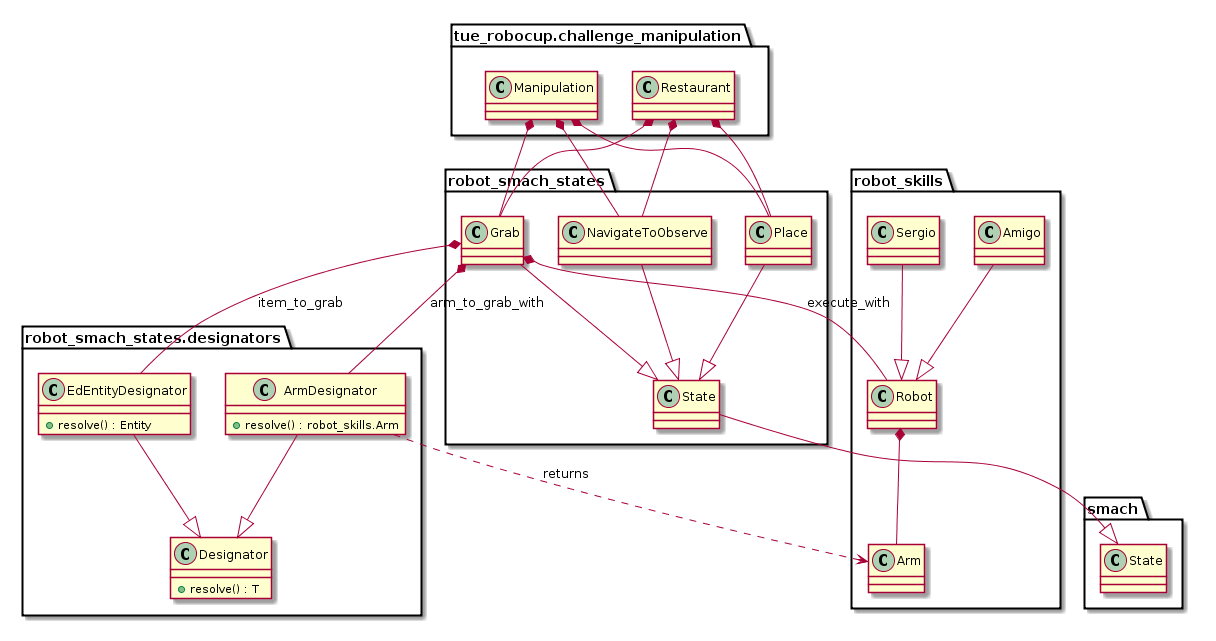
\includegraphics[width=0.9\textwidth]{robot_skill_states.png}
  \caption{Example interaction robot layers}\label{fig:robot_states_skills}
\end{figure*}

The model of the robot and requirements are created in CIF 3~\cite{cif3} and based on them a supervisor was synthesized. 
The CIF 3 language is designed to efficiently describe a plant, in this case Amigo, and its requirements, with automata or state-based expressions.
An example plant automaton is shown in \cref{code:armCIF} of Appendix~\ref{sec:code}. 
\todo[disable]{all models that are relevant or different, show skill task safety}
One recognizes the locations, including the initial and marked keywords, transitions represented by edges and declarations of (un-)controllable events as mentioned in \cref{sec:supervisory_control}.
This CIF automaton is shown graphically in \cref{fig:automaton_arm_l}.
An example of a requirement automaton in CIF and its graphical representation are shown in, respectively, \cref{code:safeArmCIF} of Appendix~\ref{sec:code} and \cref{fig:automaton_safe_arm_l}.
This safety requirement prevents collisions of the arms.
When a collision is detected on the path planned by the robot, the supervisor cancels the current plan and plans a new one.
A more detailed explanation of these models can be found in~\cite{jorrit_github}.
For this paper a set of models and requirements was created, that contained all the necessary components to execute the case studies, this can be expanded on in later research.\\

CIF uses the algorithm~\cite{CIF_algo} to synthesize a maximal permissive, controllable and non-blocking supervisor.
The output of the CIF synthesis procedure is a supervisor described in the CIF modelling language, but the CIF tool set provides conversions to other languages as well~\cite{cif3_c99}.
To integrate this supervisor with the robot and the existing control implementation, the supervisor was converted to \texttt{C} code, utilizing the tool from~\cite{cif3_c99}.
The CIF converted \texttt{C} code is available to the user as a library, which is used in this paper as follows:
the CIF generated supervisor library exposes two entry point functions to the user: \texttt{void EngineFirstStep()} and \texttt{void EngineTimeStep()}.
\texttt{void EngineFirstStep()} initializes all the data and executes the events that are not blocked by the supervisor, before the first time step.
\texttt{void EngineTimeStep(double delta)}, which needs to be called regularly by the user, updates time-dependent equations and variables in the model with time \texttt{delta} and then executes the events that are not blocked by the supervisor.
Guards for these events can depend on variables that can be set by the user, by calling a function with the name of the variable.
Looking at the example in \cref{fig:automaton_arm_l,fig:automaton_safe_arm_l}, the variables that can be set from the calling program are: \texttt{collision\_on\_path} (\(cp\)), \texttt{path\_valid} (\(pv\)) and \texttt{goal\_reached} (\(gr\)).
The function names would be, respectively, \texttt{void collision\_on\_path()}, \texttt{void path\_valid()} and \texttt{void goal\_reached()}.\\
The supervisor needs to interact with the robot, so the robot actually executes the actions imposed by the events of the supervisor.
To this end, the CIF generated supervisor library exposes a callback function \texttt{void InfoEvent(Event\_ event, BoolType pre)}.
This callback function needs to be defined in the program using the library and is called every time an event is about to, or has been executed.
In the case studies described in this paper, the function is defined in python and will execute the \texttt{robot\_states} or \texttt{robot\_skills} relevant to the event.
This function definition and other communication functions between the supervisor and the existing robot control are implemented in a file called the python wrapper.
It is important to note that to ensure that the supervisor knows if the robot is actually executing, or has completed, the task requested by the supervisor, variables need to be included so the robot can report back its current state.
CIF provides the \texttt{input} variable type, to facilitate this.
These are variables that the robot needs to assign to, after every time step, using the function \texttt{AssignInputVariables}\\
 
The complete code containing the CIF models, the supervisor and the python wrapper of the case studies, and a detailed plan on how to compile them, can be found in the code repository~\cite{jorrit_github} of the project described in this paper.
The repository also contains a detailed usage description of the CIF models, the supervisor, the python wrapper and the SMACH implementation, so the method can easily be integrated in further research.\\

Concerning the application scope of supervisory control in the case studies, the supervisor can be applied to different abstraction levels.
Applying supervisory control to the low-level control of the robot is difficult, because the control is mainly continuous and not discrete-event based.
The lowest level of abstraction supervisory control was applied to in this research was on the skill level, using the skill requirements. 
They control one component of the robot, but only the discrete events of that component.
This abstraction level was chosen, because the skills can still be described by finite-state machines and are discrete-event based.
One level of abstraction higher are the safety requirements. 
They can span multiple components and block events from one component based on information from another. 
The highest abstraction level supervisory control was applied to in this research was on the task level, using the task requirements.
They only control the order of skill events the robot executes and control nothing of the skills themselves.\\

\subsection{LIMITATIONS}
The presented case studies and method show the benefits that supervisory control synthesis can offer to autonomous robots.
There are, however, properties or benefits supervisory control synthesis can offer, that could not be translated to the dynamic environment of autonomous robots.\\

Non-blockingness, for example, can be used to ensure that a system is able to reach a certain state.
In robotics this could mean that a robot would never execute an action that would block a path, the robot later needs to navigate.
Another example where the non-blockingness property could prove useful, is a low-level implementation of supervisory control synthesis for control of the arms.
One can imagine it could be beneficial to make sure the arms never block each other when reaching for an object.
Both of these examples are impossible to implement with the method described in this paper, because of the dynamic environment the robot operates in.
This is caused by the fact that the supervisor is synthesised off-line and therefore cannot predict what happens when the robot enters an unknown environment.
There exist on-line supervisory control synthesis techniques~\cite{online_partially_observed,online_near_optimal,online_sup_rep_obs_sub}, that could prove useful in future research.\\

Another limitation is that CIF is a clear and concise language, but also somewhat limited.
Strings are not allowed as variables when performing supervisory control synthesis, for example, which is a big limitation when trying to describe a list of items to be picked up.\\%design choices
\section{RESULTS}\label{sec:results}
The case studies presented in \cref{sec:case_studies}, using the method presented in \cref{sec:method}, were implemented on the Amigo robot.
Due to the system architecture already in place, the case studies could only be partly implemented.
It was thought that the existing SMACH finite-state machines of the robot system architecture, would provide an easy platform on which to integrate the supervisor.
However, the synchronous nature of these finite-state machines and their complexity, made it difficult to integrate them with the asynchronous callback structure of the supervisor.
An example of this is the grab skill SMACH finite-state machine in the Amigo repository.
The state machine navigates the robot in front of the specified object, updates the world model, opens and closes the grabber and more.
During the execution of this state machine the supervisor cannot call other events, but without all these steps the object will not be grabbed correctly.
These are just limitations on the robot side, however, and not limitations to the applicability and benefits of supervisory control synthesis to autonomous robot.
Furthermore, future research can solve these issues by, for example, making the callbacks multi-threaded.\\

Because of these limitations case study II could not be implemented on the robot, because the current architecture only allows planning of one arm at the same time.
Case study I was implemented for the most part.

More information on what is implemented and what is not, is provided in this paper's repository~\cite{jorrit_github}.
This implementation confirmed the following benefits the method in this paper discusses:\\

\begin{LaTeXdescription}
	\item [Concurrency] In case study I the robot moves one of the arms and navigates to a table at the same time.
	\item [Modularity and Re-usability] Both case studies combine a robot model, safety requirements, skill requirements and a task requirement from which a supervisor is synthesized. When the task requirement describing case study I is replaced with the task requirement describing case study II, synthesis provides a supervisor that executes this new task.\\
\end{LaTeXdescription}

And to a lesser extent:
\begin{LaTeXdescription}
	\item [Separation] Because the safety requirements were the same for both case studies, the effect of changing a requirement was not shown. Because of the modular design, however, this property should still hold.\\
\end{LaTeXdescription}




\section{CONCLUDING REMARKS}\label{sec:conclusions}

In this paper, the limitations, the impact and benefits supervisory control synthesis can have in autonomous robots, are explored.
To this end, two case studies are described, using the Amigo robot at the Eindhoven University of Technology. 
A method is presented that can be used as a basis for implementation of supervisory control synthesis in autonomous robots.
This method defines on what abstraction levels supervisory control synthesis can be applied in autonomous robots and presents a framework for future research in the field.
The two case studies show that applying this method to autonomous robots indeed provides benefits in both system design and task execution.\\
\todo[disable]{limitations non-blocking}
Further research can increase the impact of supervisory control synthesis, by removing limitations mentioned in this paper.
On-line synthesis of the supervisor~\cite{online_partially_observed,online_near_optimal,online_sup_rep_obs_sub} increases its capability of reacting to changes in the dynamic environment of the robot.
Furthermore, using a non-monolithic supervisor is useful when the complexity and size of the system increases e.g.\@ modular~\cite{modular} or hierarchical~\cite{hierachical} synthesis.
Further research can also expand the implementaton of the case studies described in this paper, to provide further insight into the application of supervisory control synthesis to autonomous robots.\\

\todo[disable]{talk about making supervisor from modular requirements, coordinator and checking}
\section*{ACKNOWLEDGEMENT} The authors would like to thank Albert Hofkamp, as he has been an enormous help in understanding the CIF tool set and providing a way to convert a CIF specification into a working supervisor implementation in \texttt{C}.\\
\printbibliography{} 
\newpage
\appendices
\section{CIF AUTOMATA:\@ GRAPHICAL}\label{sec:model_req}

\begin{figure}[!ht]
  \begin{center}
  \begin{tikzpicture}[->,>=stealth',shorten >=1pt,auto,node distance=3cm,
                      semithick, font=\footnotesize]
    % \tikzstyle{every state}=[fill=red,draw=none,text=white]

    \node[state,accepting]              (1)                     {$idling$};
    \node[state, accepting]             (2) [align=center,left of=1]         {$planning$};
    \node[state, accepting]             (3) [align=center,right of=1]        {$planning$\\ $to\ grab$};
    \node[state, accepting]             (4) [align=center,below of=2]        {$moving$};
    \node[state,accepting]              (5) [align=center, below of=3]  {$grabbing$};
    \node[state,accepting]              (6) [align=center, below=3.5cm of 1]  {$re$-\\$planning$} ;

    \draw[<-] (1) -- node {} ++(0,2cm);


    \path (1) edge []          node [align=center, above]       {$plan$} (2)
              edge [bend left]          node [align=center, above]      {$plan\ to\ grab$}   (3)
          (2) edge [bend right]          node [align=center, left]             {$move$}   (4)
              edge [bend left]          node [align=center, above]    {$idle$}   (1)
          (3) edge [bend left]          node [align=center]             {$grab$}   (5)
              edge []          node [align=center, above]             {$idle$}   (1)
          (4) edge [bend left]          node [align=center, left]       {$replan$}   (6)
              edge []                   node [align=center, below, pos=0.25]      {$plan$\\$to\ grab$}   (3)
              edge []          node [align=center, left,pos=0.4]      {$gr\ \|\ !ma$\\$idle$}   (1)
          (5) edge []                   node [align=center, below, pos=0.25]       {$plan$}   (2)
              edge [bend left]          node [align=center, below]      {$replan$}   (6)
              edge []          node [align=center, right,pos=0.4]      {$oa\ \|\ !ma$\\$idle$}   (1)
          (6) edge [bend left]          node [align=left, right]             {$grab$}   (5)
              edge []          node [align=center, left, pos=0.9]             {$idle$}   (1)
              edge [bend left]          node [align=center]             {$move$}   (4);
  \end{tikzpicture}
  \caption{Automaton of left arm}
  \label{fig:automaton_arm_l}
  \end{center}
with:
\begin{description}
  \item[\(gr\)] goal reached
  \item[\(ma\)] moving arm
  \item[\(oa\)] object in arm\\
\end{description}
\end{figure}

\begin{figure}[!ht]
  \begin{center}
  \begin{tikzpicture}[->,>=stealth',shorten >=1pt,auto,node distance=6cm,
                      semithick, font=\footnotesize]
    % \tikzstyle{every state}=[fill=red,draw=none,text=white]

    \node[state,accepting]      (1)                     {};


    \path (1) edge [loop above]          node [align=center]       {$pv=1\ \&\&\ !cp$ \\ $arm.move$} ()
              edge [loop left]          node [align=center]       {$pv\ !=1\ \|\ cp$ \\ $arm.replan$} ()
              edge [loop right]          node [align=center]       {$pv=2\ \|\ gr\ \|\ !am$ \\ $arm.idle$} ()
              edge [loop below]          node [align=center]       {$pv=1\ \&\&\ !cp$ \\ $arm.grab$} ();
  \end{tikzpicture}
  \caption{Automaton of safety requirement left arm}

  \label{fig:automaton_safe_arm_l}
\end{center}
with:
\begin{description}
  \item[\(pv\)] plan viable
  \item[\(cp\)] collision on path
  \item[\(gr\)] goal reached
  \item[\(!am\)] arm.moving-arm = false, while arm is in location moving\\
\end{description}
\end{figure}

% controllable goto_phase2;

% requirement task:
%    controllable waiting;
% //     disc list string nav_waypoints = [""];
% //     disc list string objects_to_grab = [""];
%     input bool object_grabbed;
%     disc bool navigating = false;
%     disc bool grabbing = false;

%     location phase1:
%     initial;
%     marked;
% //      edge grab_skill.write when start = true do start := false;
%     edge navigation_skill.move_to when navigating = false do navigating := true;
%     edge grab_skill.grab when grabbing = false do grabbing := true;
%     edge waiting when navigating = true and grabbing = true goto wait;

%     location wait:
%     marked;
%     edge goto_phase2 when object_grabbed = true goto phase2;

%     location phase2:
%     marked;
% //      grab_skill.place_point := "table2"
%     edge navigation_skill.move_to;// do navigate.waypoint := "table2";
% //      edge grab_skill.release;// when; \\There is a table?


 % location phase2:
 %    marked;
 %    edge navigation_skill.move_to when navigating = false do navigating := true;
 %    edge place_skill.release when grabbing = false do grabbing := true;
% end

\begin{figure}[!ht]
  \begin{center}
  \begin{tikzpicture}[->,>=stealth',shorten >=1pt,auto,node distance=3cm,
                      semithick, font=\footnotesize]
    % \tikzstyle{every state}=[fill=red,draw=none,text=white]

    \node[state, accepting]             (1)                                  {$phase1$};
    \node[state, accepting]             (2) [align=center,below of=1]         {$wait$};
    \node[state, accepting]             (3) [align=center,below of=2]        {$phase2$};


    \draw[<-] (1) -- node {} ++(0,2cm);


    \path (1) edge [loop right]         node [align=center, right]       {$!nv$ \\ $navigation\_skill.move\_to$ \\ $nv := true$} ()
              edge [loop left]          node [align=center, left]      {$!gr$ \\ $grab\_skill.grab$ \\ $gr := true$}   ()
              edge []                   node [align=center]      {$nv\ \&\&\ gr$ \\ $waiting$} (2)
          (2) edge []                   node [align=center]            {$og$ \\ $goto\_phase$2 \\ $nv := false\ \&\&\ gr := false$} (3)
          (3) edge [loop right]         node [align=center, right]       {$!nv$ \\ $navigation\_skill.move\_to$ \\ $nv := true$} ()
              edge [loop left]          node [align=center, left]      {$!gr$ \\ $place\_skill.release$ \\ $gr := true$}   ();

  \end{tikzpicture}
  \caption{Automaton of pick-up task}
  \label{fig:pick_task}
  \end{center}
with:
\begin{description}
  \item[\(nv\)] navigating
  \item[\(gr\)] grabbing
  \item[\(og\)] object grabbed\\
\end{description}
\end{figure}


\newpage
\section{CIF AUTOMATA:\@ CODE}\label{sec:code}

\begin{center}
\begin{minipage}{0.95\columnwidth}
% \begin{tabular}{c}
\begin{lstlisting}[caption=CIF model of pick-up task requirement, label=code:pick_task, language=CIF]%, linewidth=0.8\columnwidt

requirement task:
   controllable waiting, goto_phase2;

    input bool object_grabbed;
    disc bool navigating = false;
    disc bool grabbing = false;

    location phase1:
    initial;
    marked;
    edge navigation_skill.move_to when navigating = false do navigating := true;
    edge grab_skill.grab when grabbing = false do grabbing := true;
    edge waiting when navigating = true and grabbing = true do navigating := false and grabbing := false goto wait;

    location wait:
    marked;
    edge goto_phase2 when object_grabbed = true goto phase2;

    location phase2:
    marked;
    edge navigation_skill.move_to when navigating = false do navigating := true;
    edge place_skill.release when grabbing = false do grabbing := true;
end
\end{lstlisting}
\end{minipage}
% \end{tabular}
\end{center}


\begin{center}
\begin{minipage}{0.95\columnwidth}
% \begin{tabular}{c}
\begin{lstlisting}[caption=CIF model of safety requirement arms, label=code:safeArmCIF, language=CIF]%, linewidth=0.8\columnwidt

requirement def SafeArmMovement(Arm arm):
    location:
    initial;
    marked;
    edge arm.replan when arm.collision_on_path or arm.plan_viable != 1;
    edge arm.move when arm.plan_viable = 1 and not arm.collision_on_path;
    edge arm.grab when arm.plan_viable = 1 and not arm.collision_on_path;
    edge arm.idle when arm.plan_viable = 2 or arm.goal_reached or arm.moving_arm != true; // Set plan_viable to 0
end

requirement_arm_left: SafeArmMovement(arm_left);
requirement_arm_right: SafeArmMovement(arm_right);

\end{lstlisting}
\end{minipage}
% \end{tabular}
\end{center}

\begin{center}
\begin{minipage}{0.95\columnwidth}
% \begin{tabular}{c}
\begin{lstlisting}[caption=CIF model of grab skill requirement, label=code:grab_skill, language=CIF]%, linewidth=0.8\columnwidt

requirement grab_skill:
    controllable grab, determine_grab_arm;

    input int [0..2] use_arm; //0 nothing, 1 left, 2 right

    location idling:
    initial;
    marked;
    edge grab goto grabbing;

    location grabbing:
    marked;
    edge determine_grab_arm when use_arm = 0;
    edge left_grab_exec.start when use_arm = 1 goto idling;
    edge right_grab_exec.start when use_arm = 2 goto idling;
end

requirement def grab_exec(Arm arm):
    controllable check_in_WS, start, complete, idle;

    input int [0..2] object_in_WS;

    location idling:
    initial;
    marked;
    edge start goto starting;

    location starting:
    marked;
    edge check_in_WS when object_in_WS = 0;
    edge arm.plan when object_in_WS = 1;
    edge arm.plan_to_grab when object_in_WS = 2;
    edge complete when arm.object_in_arm goto completing;

    location completing:
    marked;
    edge idle goto idling;

end

left_grab_exec: grab_exec(arm_left);
right_grab_exec: grab_exec(arm_right);
\end{lstlisting}
\end{minipage}
% \end{tabular}
\end{center}

\begin{center}
\begin{minipage}{0.95\columnwidth}
% \begin{tabular}{c}
\begin{lstlisting}[caption=CIF model of Amigo Arms, label=code:armCIF, language=CIF]%, linewidth=0.8\columnwidth]

plant automaton def Arm():
    // Events
    // Stop all movement, move arm to plan, plan to waypoint
    controllable idle, move, plan, replan, plan_to_grab, grab;

    // Variables
    input int [0..2] plan_viable; //{0,1,2} = {empty,true,false}
    input bool collision_on_path;
    input bool moving_arm;
    input bool goal_reached;
    input bool object_in_arm;

    location idling:
    marked;
    initial;
    edge plan goto planning;
    edge plan_to_grab goto planning_to_grab;

    location planning:
    // entry point to start moving to something
    marked;
    edge move goto moving;
    edge idle goto idling;

    location planning_to_grab:
    marked;
    edge grab goto grabbing;
    edge idle goto idling;

    location replanning:
    marked;
    edge move goto moving;
    edge grab goto grabbing;
    edge idle goto idling;

    location moving:
    marked;
    edge plan_to_grab goto planning_to_grab;
    edge replan goto replanning;
    edge idle when (goal_reached or moving_arm != true) goto idling;

    location grabbing:
    marked;
    edge plan goto planning;
    edge replan goto replanning;
    edge idle when (object_in_arm or moving_arm != true) goto idling;

end

arm_left: Arm();
arm_right: Arm();
\end{lstlisting}
\end{minipage}
% \end{tabular}
\end{center}


\end{document}
